% Options for packages loaded elsewhere
\PassOptionsToPackage{unicode}{hyperref}
\PassOptionsToPackage{hyphens}{url}
\PassOptionsToPackage{dvipsnames,svgnames,x11names}{xcolor}
%
\documentclass[
  letterpaper,
  DIV=11,
  numbers=noendperiod]{scrartcl}

\usepackage{amsmath,amssymb}
\usepackage{iftex}
\ifPDFTeX
  \usepackage[T1]{fontenc}
  \usepackage[utf8]{inputenc}
  \usepackage{textcomp} % provide euro and other symbols
\else % if luatex or xetex
  \usepackage{unicode-math}
  \defaultfontfeatures{Scale=MatchLowercase}
  \defaultfontfeatures[\rmfamily]{Ligatures=TeX,Scale=1}
\fi
\usepackage{lmodern}
\ifPDFTeX\else  
    % xetex/luatex font selection
\fi
% Use upquote if available, for straight quotes in verbatim environments
\IfFileExists{upquote.sty}{\usepackage{upquote}}{}
\IfFileExists{microtype.sty}{% use microtype if available
  \usepackage[]{microtype}
  \UseMicrotypeSet[protrusion]{basicmath} % disable protrusion for tt fonts
}{}
\makeatletter
\@ifundefined{KOMAClassName}{% if non-KOMA class
  \IfFileExists{parskip.sty}{%
    \usepackage{parskip}
  }{% else
    \setlength{\parindent}{0pt}
    \setlength{\parskip}{6pt plus 2pt minus 1pt}}
}{% if KOMA class
  \KOMAoptions{parskip=half}}
\makeatother
\usepackage{xcolor}
\setlength{\emergencystretch}{3em} % prevent overfull lines
\setcounter{secnumdepth}{-\maxdimen} % remove section numbering
% Make \paragraph and \subparagraph free-standing
\ifx\paragraph\undefined\else
  \let\oldparagraph\paragraph
  \renewcommand{\paragraph}[1]{\oldparagraph{#1}\mbox{}}
\fi
\ifx\subparagraph\undefined\else
  \let\oldsubparagraph\subparagraph
  \renewcommand{\subparagraph}[1]{\oldsubparagraph{#1}\mbox{}}
\fi

\usepackage{color}
\usepackage{fancyvrb}
\newcommand{\VerbBar}{|}
\newcommand{\VERB}{\Verb[commandchars=\\\{\}]}
\DefineVerbatimEnvironment{Highlighting}{Verbatim}{commandchars=\\\{\}}
% Add ',fontsize=\small' for more characters per line
\usepackage{framed}
\definecolor{shadecolor}{RGB}{241,243,245}
\newenvironment{Shaded}{\begin{snugshade}}{\end{snugshade}}
\newcommand{\AlertTok}[1]{\textcolor[rgb]{0.68,0.00,0.00}{#1}}
\newcommand{\AnnotationTok}[1]{\textcolor[rgb]{0.37,0.37,0.37}{#1}}
\newcommand{\AttributeTok}[1]{\textcolor[rgb]{0.40,0.45,0.13}{#1}}
\newcommand{\BaseNTok}[1]{\textcolor[rgb]{0.68,0.00,0.00}{#1}}
\newcommand{\BuiltInTok}[1]{\textcolor[rgb]{0.00,0.23,0.31}{#1}}
\newcommand{\CharTok}[1]{\textcolor[rgb]{0.13,0.47,0.30}{#1}}
\newcommand{\CommentTok}[1]{\textcolor[rgb]{0.37,0.37,0.37}{#1}}
\newcommand{\CommentVarTok}[1]{\textcolor[rgb]{0.37,0.37,0.37}{\textit{#1}}}
\newcommand{\ConstantTok}[1]{\textcolor[rgb]{0.56,0.35,0.01}{#1}}
\newcommand{\ControlFlowTok}[1]{\textcolor[rgb]{0.00,0.23,0.31}{#1}}
\newcommand{\DataTypeTok}[1]{\textcolor[rgb]{0.68,0.00,0.00}{#1}}
\newcommand{\DecValTok}[1]{\textcolor[rgb]{0.68,0.00,0.00}{#1}}
\newcommand{\DocumentationTok}[1]{\textcolor[rgb]{0.37,0.37,0.37}{\textit{#1}}}
\newcommand{\ErrorTok}[1]{\textcolor[rgb]{0.68,0.00,0.00}{#1}}
\newcommand{\ExtensionTok}[1]{\textcolor[rgb]{0.00,0.23,0.31}{#1}}
\newcommand{\FloatTok}[1]{\textcolor[rgb]{0.68,0.00,0.00}{#1}}
\newcommand{\FunctionTok}[1]{\textcolor[rgb]{0.28,0.35,0.67}{#1}}
\newcommand{\ImportTok}[1]{\textcolor[rgb]{0.00,0.46,0.62}{#1}}
\newcommand{\InformationTok}[1]{\textcolor[rgb]{0.37,0.37,0.37}{#1}}
\newcommand{\KeywordTok}[1]{\textcolor[rgb]{0.00,0.23,0.31}{#1}}
\newcommand{\NormalTok}[1]{\textcolor[rgb]{0.00,0.23,0.31}{#1}}
\newcommand{\OperatorTok}[1]{\textcolor[rgb]{0.37,0.37,0.37}{#1}}
\newcommand{\OtherTok}[1]{\textcolor[rgb]{0.00,0.23,0.31}{#1}}
\newcommand{\PreprocessorTok}[1]{\textcolor[rgb]{0.68,0.00,0.00}{#1}}
\newcommand{\RegionMarkerTok}[1]{\textcolor[rgb]{0.00,0.23,0.31}{#1}}
\newcommand{\SpecialCharTok}[1]{\textcolor[rgb]{0.37,0.37,0.37}{#1}}
\newcommand{\SpecialStringTok}[1]{\textcolor[rgb]{0.13,0.47,0.30}{#1}}
\newcommand{\StringTok}[1]{\textcolor[rgb]{0.13,0.47,0.30}{#1}}
\newcommand{\VariableTok}[1]{\textcolor[rgb]{0.07,0.07,0.07}{#1}}
\newcommand{\VerbatimStringTok}[1]{\textcolor[rgb]{0.13,0.47,0.30}{#1}}
\newcommand{\WarningTok}[1]{\textcolor[rgb]{0.37,0.37,0.37}{\textit{#1}}}

\providecommand{\tightlist}{%
  \setlength{\itemsep}{0pt}\setlength{\parskip}{0pt}}\usepackage{longtable,booktabs,array}
\usepackage{calc} % for calculating minipage widths
% Correct order of tables after \paragraph or \subparagraph
\usepackage{etoolbox}
\makeatletter
\patchcmd\longtable{\par}{\if@noskipsec\mbox{}\fi\par}{}{}
\makeatother
% Allow footnotes in longtable head/foot
\IfFileExists{footnotehyper.sty}{\usepackage{footnotehyper}}{\usepackage{footnote}}
\makesavenoteenv{longtable}
\usepackage{graphicx}
\makeatletter
\def\maxwidth{\ifdim\Gin@nat@width>\linewidth\linewidth\else\Gin@nat@width\fi}
\def\maxheight{\ifdim\Gin@nat@height>\textheight\textheight\else\Gin@nat@height\fi}
\makeatother
% Scale images if necessary, so that they will not overflow the page
% margins by default, and it is still possible to overwrite the defaults
% using explicit options in \includegraphics[width, height, ...]{}
\setkeys{Gin}{width=\maxwidth,height=\maxheight,keepaspectratio}
% Set default figure placement to htbp
\makeatletter
\def\fps@figure{htbp}
\makeatother

\KOMAoption{captions}{tableheading}
\makeatletter
\makeatother
\makeatletter
\makeatother
\makeatletter
\@ifpackageloaded{caption}{}{\usepackage{caption}}
\AtBeginDocument{%
\ifdefined\contentsname
  \renewcommand*\contentsname{Table of contents}
\else
  \newcommand\contentsname{Table of contents}
\fi
\ifdefined\listfigurename
  \renewcommand*\listfigurename{List of Figures}
\else
  \newcommand\listfigurename{List of Figures}
\fi
\ifdefined\listtablename
  \renewcommand*\listtablename{List of Tables}
\else
  \newcommand\listtablename{List of Tables}
\fi
\ifdefined\figurename
  \renewcommand*\figurename{Figure}
\else
  \newcommand\figurename{Figure}
\fi
\ifdefined\tablename
  \renewcommand*\tablename{Table}
\else
  \newcommand\tablename{Table}
\fi
}
\@ifpackageloaded{float}{}{\usepackage{float}}
\floatstyle{ruled}
\@ifundefined{c@chapter}{\newfloat{codelisting}{h}{lop}}{\newfloat{codelisting}{h}{lop}[chapter]}
\floatname{codelisting}{Listing}
\newcommand*\listoflistings{\listof{codelisting}{List of Listings}}
\makeatother
\makeatletter
\@ifpackageloaded{caption}{}{\usepackage{caption}}
\@ifpackageloaded{subcaption}{}{\usepackage{subcaption}}
\makeatother
\makeatletter
\@ifpackageloaded{tcolorbox}{}{\usepackage[skins,breakable]{tcolorbox}}
\makeatother
\makeatletter
\@ifundefined{shadecolor}{\definecolor{shadecolor}{rgb}{.97, .97, .97}}
\makeatother
\makeatletter
\makeatother
\makeatletter
\makeatother
\ifLuaTeX
  \usepackage{selnolig}  % disable illegal ligatures
\fi
\IfFileExists{bookmark.sty}{\usepackage{bookmark}}{\usepackage{hyperref}}
\IfFileExists{xurl.sty}{\usepackage{xurl}}{} % add URL line breaks if available
\urlstyle{same} % disable monospaced font for URLs
\hypersetup{
  pdftitle={Class 7: Machine Learning 1},
  pdfauthor={Raquel Gonzalez (PID: A16207442)},
  colorlinks=true,
  linkcolor={blue},
  filecolor={Maroon},
  citecolor={Blue},
  urlcolor={Blue},
  pdfcreator={LaTeX via pandoc}}

\title{Class 7: Machine Learning 1}
\author{Raquel Gonzalez (PID: A16207442)}
\date{}

\begin{document}
\maketitle
\ifdefined\Shaded\renewenvironment{Shaded}{\begin{tcolorbox}[sharp corners, borderline west={3pt}{0pt}{shadecolor}, interior hidden, enhanced, breakable, boxrule=0pt, frame hidden]}{\end{tcolorbox}}\fi

\hypertarget{clustering-methods}{%
\section{Clustering Methods}\label{clustering-methods}}

The broad goal here is to find groupings (clusters) in your input data.

\hypertarget{kmeans}{%
\subsection{Kmeans}\label{kmeans}}

First, let's make up some data to cluster.

\begin{Shaded}
\begin{Highlighting}[]
\NormalTok{x }\OtherTok{\textless{}{-}} \FunctionTok{rnorm}\NormalTok{(}\DecValTok{1000}\NormalTok{)}
\FunctionTok{hist}\NormalTok{(x)}
\end{Highlighting}
\end{Shaded}

\begin{figure}[H]

{\centering 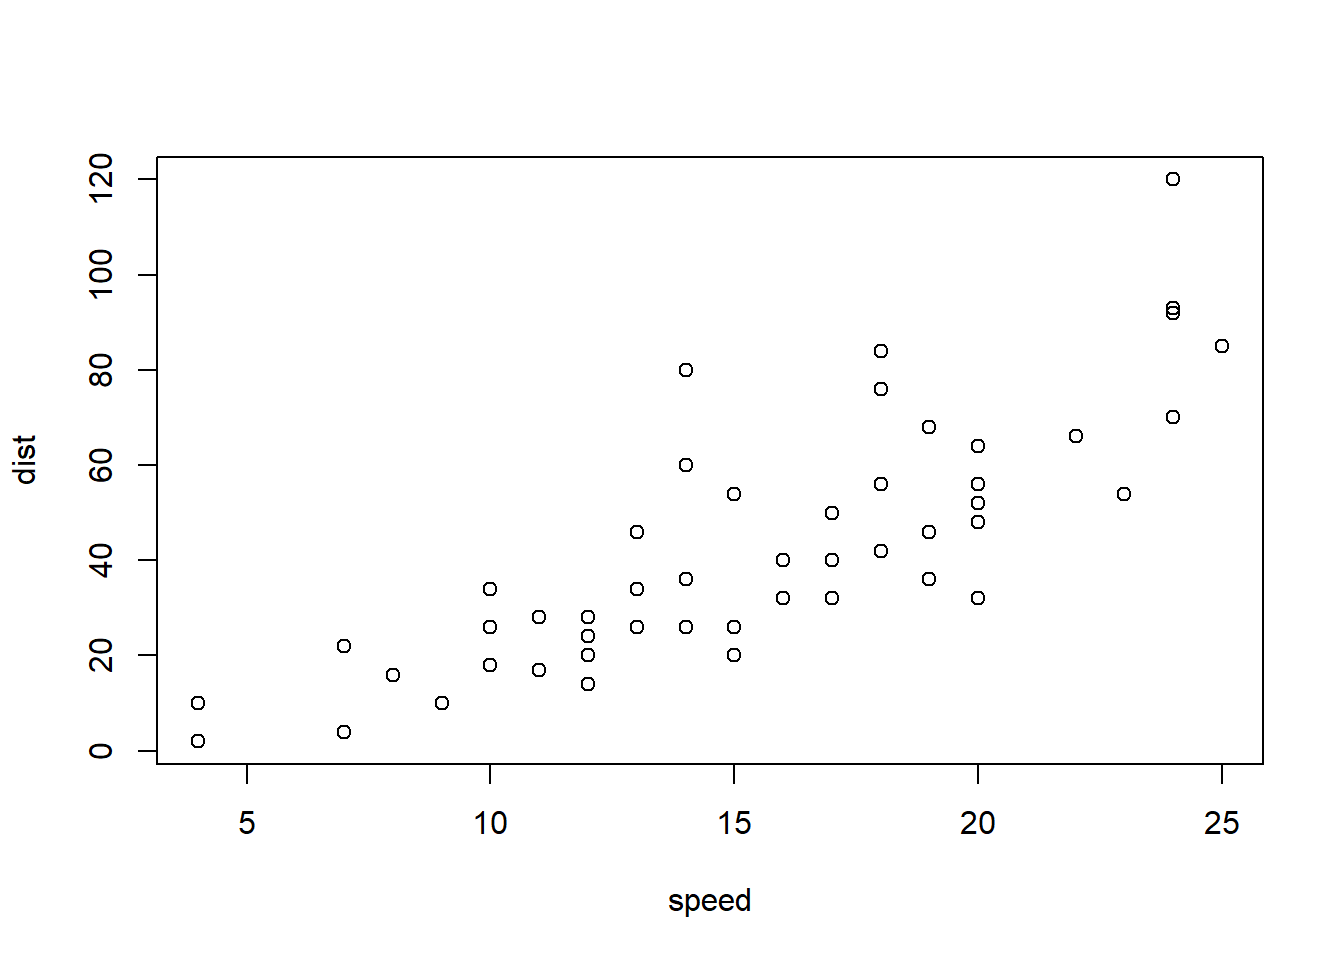
\includegraphics{class07_files/figure-pdf/unnamed-chunk-1-1.pdf}

}

\end{figure}

Make a vector of length 60 with 30 points centered at -3 and 30 points
centered at +3.

\begin{Shaded}
\begin{Highlighting}[]
\NormalTok{tmp }\OtherTok{\textless{}{-}} \FunctionTok{c}\NormalTok{(}\FunctionTok{rnorm}\NormalTok{(}\DecValTok{30}\NormalTok{, }\AttributeTok{mean=}\SpecialCharTok{{-}}\DecValTok{3}\NormalTok{), }\FunctionTok{rnorm}\NormalTok{(}\DecValTok{30}\NormalTok{, }\AttributeTok{mean=}\DecValTok{3}\NormalTok{))}
\end{Highlighting}
\end{Shaded}

I will now make a wee x and y dataset with 2 groups of points

\begin{Shaded}
\begin{Highlighting}[]
\NormalTok{x }\OtherTok{\textless{}{-}} \FunctionTok{cbind}\NormalTok{(}\AttributeTok{x=}\NormalTok{tmp, }\AttributeTok{y=}\FunctionTok{rev}\NormalTok{(tmp))}
\FunctionTok{plot}\NormalTok{(x)}
\end{Highlighting}
\end{Shaded}

\begin{figure}[H]

{\centering 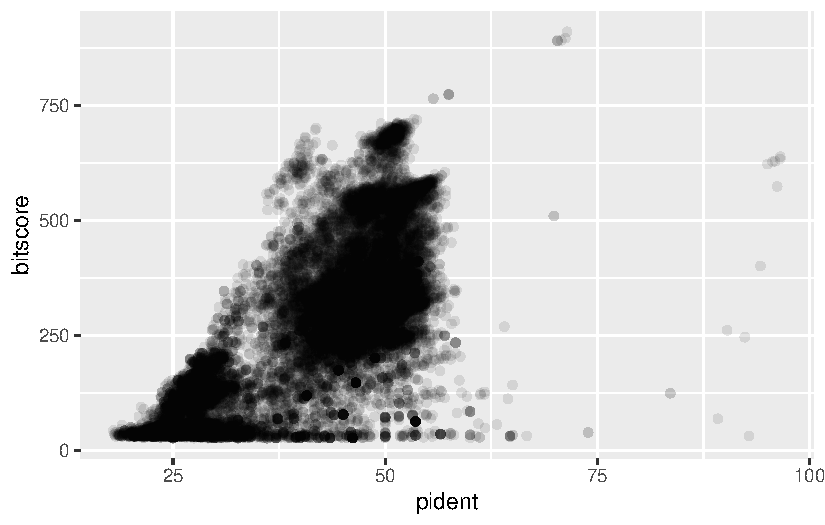
\includegraphics{class07_files/figure-pdf/unnamed-chunk-3-1.pdf}

}

\end{figure}

\begin{Shaded}
\begin{Highlighting}[]
\NormalTok{k }\OtherTok{\textless{}{-}} \FunctionTok{kmeans}\NormalTok{(x, }\AttributeTok{centers=}\DecValTok{2}\NormalTok{)}
\NormalTok{k}
\end{Highlighting}
\end{Shaded}

\begin{verbatim}
K-means clustering with 2 clusters of sizes 30, 30

Cluster means:
          x         y
1 -2.983616  3.016247
2  3.016247 -2.983616

Clustering vector:
 [1] 1 1 1 1 1 1 1 1 1 1 1 1 1 1 1 1 1 1 1 1 1 1 1 1 1 1 1 1 1 1 2 2 2 2 2 2 2 2
[39] 2 2 2 2 2 2 2 2 2 2 2 2 2 2 2 2 2 2 2 2 2 2

Within cluster sum of squares by cluster:
[1] 65.7638 65.7638
 (between_SS / total_SS =  89.1 %)

Available components:

[1] "cluster"      "centers"      "totss"        "withinss"     "tot.withinss"
[6] "betweenss"    "size"         "iter"         "ifault"      
\end{verbatim}

\begin{quote}
Q. From your result object `k', how many points are in each cluster?
\end{quote}

\begin{Shaded}
\begin{Highlighting}[]
\NormalTok{k}\SpecialCharTok{$}\NormalTok{size}
\end{Highlighting}
\end{Shaded}

\begin{verbatim}
[1] 30 30
\end{verbatim}

\begin{quote}
Q. What ``component'' of your result object details the cluster
membership?
\end{quote}

\begin{Shaded}
\begin{Highlighting}[]
\NormalTok{k}\SpecialCharTok{$}\NormalTok{cluster}
\end{Highlighting}
\end{Shaded}

\begin{verbatim}
 [1] 1 1 1 1 1 1 1 1 1 1 1 1 1 1 1 1 1 1 1 1 1 1 1 1 1 1 1 1 1 1 2 2 2 2 2 2 2 2
[39] 2 2 2 2 2 2 2 2 2 2 2 2 2 2 2 2 2 2 2 2 2 2
\end{verbatim}

\begin{quote}
Q. Cluster centers?
\end{quote}

\begin{Shaded}
\begin{Highlighting}[]
\NormalTok{k}\SpecialCharTok{$}\NormalTok{centers}
\end{Highlighting}
\end{Shaded}

\begin{verbatim}
          x         y
1 -2.983616  3.016247
2  3.016247 -2.983616
\end{verbatim}

\begin{quote}
Q. Plot of our clustering results
\end{quote}

\begin{Shaded}
\begin{Highlighting}[]
\FunctionTok{plot}\NormalTok{(x, }\AttributeTok{col=}\NormalTok{k}\SpecialCharTok{$}\NormalTok{cluster)}
\FunctionTok{points}\NormalTok{(k}\SpecialCharTok{$}\NormalTok{centers, }\AttributeTok{col=}\StringTok{"blue"}\NormalTok{, }\AttributeTok{pch=}\DecValTok{15}\NormalTok{, }\AttributeTok{cex=}\DecValTok{2}\NormalTok{)}
\end{Highlighting}
\end{Shaded}

\begin{figure}[H]

{\centering 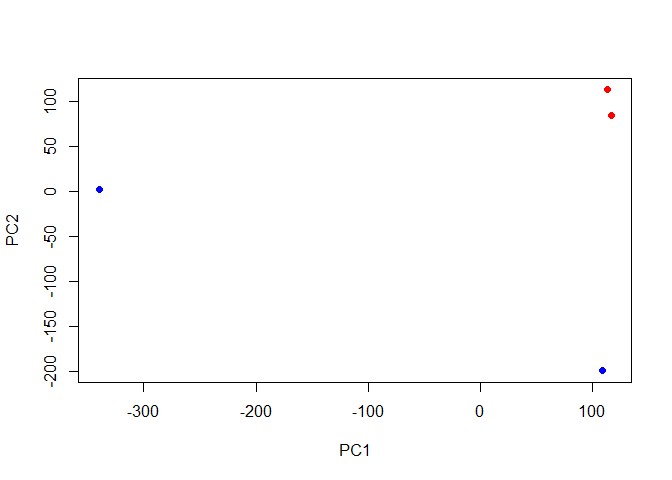
\includegraphics{class07_files/figure-pdf/unnamed-chunk-8-1.pdf}

}

\end{figure}

We can cluster data into 4 groups.

\begin{Shaded}
\begin{Highlighting}[]
\CommentTok{\# kmeans}
\NormalTok{k4 }\OtherTok{\textless{}{-}} \FunctionTok{kmeans}\NormalTok{(x, }\AttributeTok{centers=}\DecValTok{4}\NormalTok{)}
\CommentTok{\# plot results}
\FunctionTok{plot}\NormalTok{(x, }\AttributeTok{col=}\NormalTok{k4}\SpecialCharTok{$}\NormalTok{cluster)}
\end{Highlighting}
\end{Shaded}

\begin{figure}[H]

{\centering 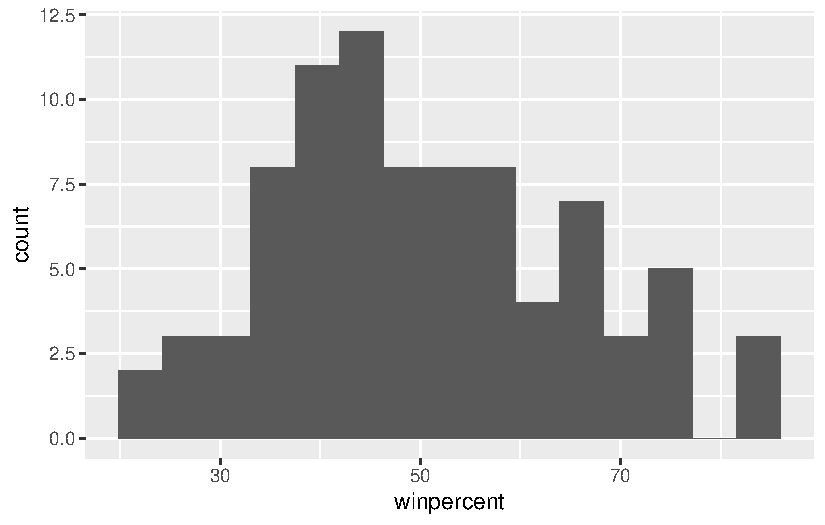
\includegraphics{class07_files/figure-pdf/unnamed-chunk-9-1.pdf}

}

\end{figure}

A big limitation of kmeans is that it does what you ask even if you ask
for silly clusters.

\hypertarget{hierarchical-clustering}{%
\subsection{Hierarchical Clustering}\label{hierarchical-clustering}}

The main base R function for Hierarchical Clustering is
\texttt{hclust()}. Unlike \texttt{kmeans()}, you cannot just pass it
your data as input. You first need to calculate a distance matrix.

\begin{Shaded}
\begin{Highlighting}[]
\NormalTok{d }\OtherTok{\textless{}{-}} \FunctionTok{dist}\NormalTok{(x)}
\NormalTok{hc }\OtherTok{\textless{}{-}} \FunctionTok{hclust}\NormalTok{(d)}
\NormalTok{hc}
\end{Highlighting}
\end{Shaded}

\begin{verbatim}

Call:
hclust(d = d)

Cluster method   : complete 
Distance         : euclidean 
Number of objects: 60 
\end{verbatim}

Use \texttt{plot()} to view results

\begin{Shaded}
\begin{Highlighting}[]
\FunctionTok{plot}\NormalTok{(hc)}
\FunctionTok{abline}\NormalTok{(}\AttributeTok{h=}\DecValTok{10}\NormalTok{, }\AttributeTok{col=}\StringTok{"red"}\NormalTok{)}
\end{Highlighting}
\end{Shaded}

\begin{figure}[H]

{\centering 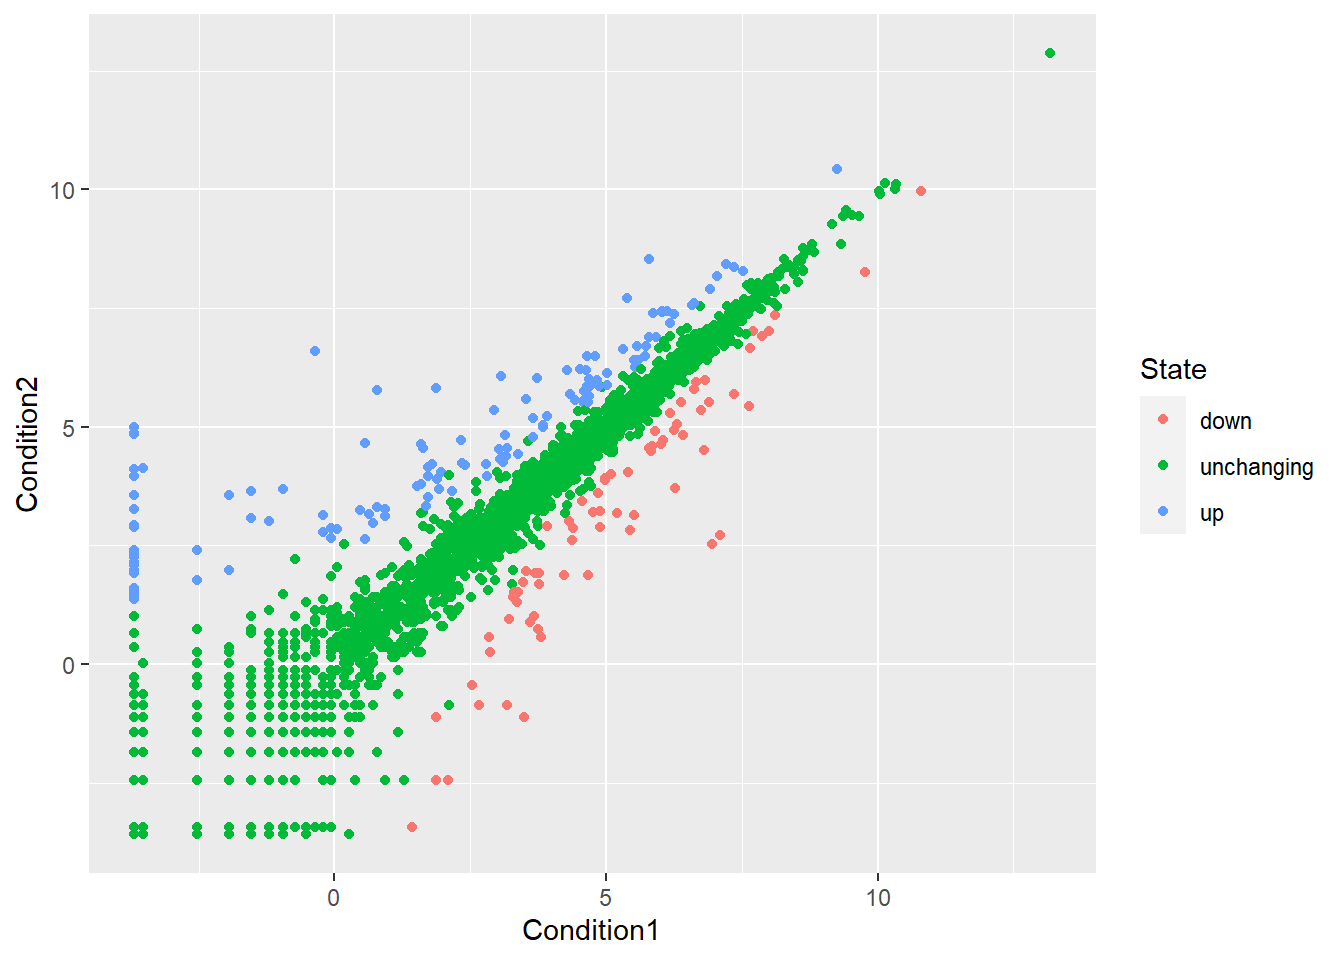
\includegraphics{class07_files/figure-pdf/unnamed-chunk-11-1.pdf}

}

\end{figure}

To make the ``cut'' and get our cluster membership vector we can use the
\texttt{cutree()} function

\begin{Shaded}
\begin{Highlighting}[]
\NormalTok{grps }\OtherTok{\textless{}{-}} \FunctionTok{cutree}\NormalTok{(hc, }\AttributeTok{h=}\DecValTok{10}\NormalTok{)}
\NormalTok{grps}
\end{Highlighting}
\end{Shaded}

\begin{verbatim}
 [1] 1 1 1 1 1 1 1 1 1 1 1 1 1 1 1 1 1 1 1 1 1 1 1 1 1 1 1 1 1 1 2 2 2 2 2 2 2 2
[39] 2 2 2 2 2 2 2 2 2 2 2 2 2 2 2 2 2 2 2 2 2 2
\end{verbatim}

Make a plot of our data colored by hclust results.

\begin{Shaded}
\begin{Highlighting}[]
\FunctionTok{plot}\NormalTok{(x, }\AttributeTok{col=}\NormalTok{grps)}
\end{Highlighting}
\end{Shaded}

\begin{figure}[H]

{\centering 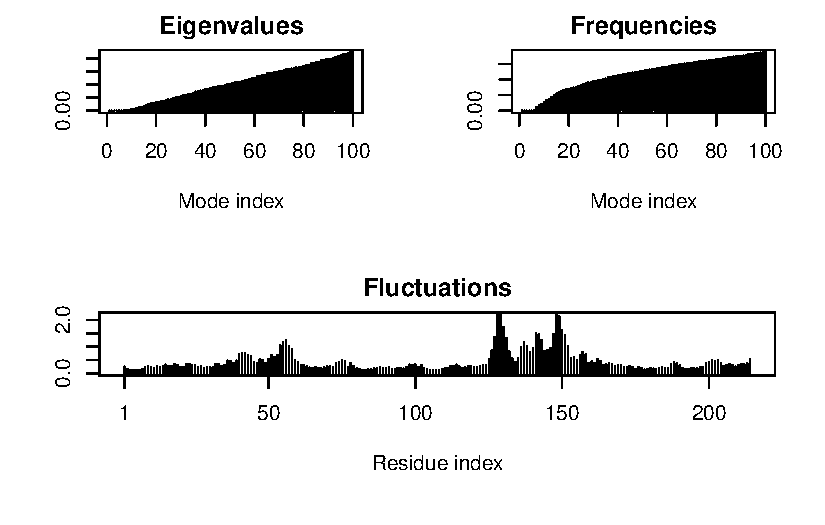
\includegraphics{class07_files/figure-pdf/unnamed-chunk-13-1.pdf}

}

\end{figure}

\hypertarget{principal-component-analysis-pca}{%
\section{Principal Component Analysis
(PCA)}\label{principal-component-analysis-pca}}

Here we will do Principal Component Analysis (PCA) on some food data
from the UK.

\begin{Shaded}
\begin{Highlighting}[]
\NormalTok{url }\OtherTok{\textless{}{-}} \StringTok{"https://tinyurl.com/UK{-}foods"}
\NormalTok{x }\OtherTok{\textless{}{-}} \FunctionTok{read.csv}\NormalTok{(url, }\AttributeTok{row.names =} \DecValTok{1}\NormalTok{)}
\end{Highlighting}
\end{Shaded}

\begin{Shaded}
\begin{Highlighting}[]
\CommentTok{\#rownames(x) \textless{}{-}  x[,1]}
\CommentTok{\#x \textless{}{-} x[, {-}1]}
\CommentTok{\#x}
\end{Highlighting}
\end{Shaded}

\begin{quote}
Q1. How many rows and columns are in your new data frame named
\texttt{x}? What R functions could you use to answer this question?
\end{quote}

\begin{Shaded}
\begin{Highlighting}[]
\FunctionTok{dim}\NormalTok{(x)}
\end{Highlighting}
\end{Shaded}

\begin{verbatim}
[1] 17  4
\end{verbatim}

\begin{Shaded}
\begin{Highlighting}[]
\DocumentationTok{\#\#Preview the first 6 rows}
\FunctionTok{head}\NormalTok{(x)}
\end{Highlighting}
\end{Shaded}

\begin{verbatim}
               England Wales Scotland N.Ireland
Cheese             105   103      103        66
Carcass_meat       245   227      242       267
Other_meat         685   803      750       586
Fish               147   160      122        93
Fats_and_oils      193   235      184       209
Sugars             156   175      147       139
\end{verbatim}

\begin{quote}
Q2: Which approach to solving the `row-names problem' mentioned above do
you prefer and why? Is one approach more robust than another under
certain circumstances?
\end{quote}

Setting the row.names argument is preferred, because the
\texttt{rownames()} function will consistently delete the first row each
time you run it.

\begin{quote}
Q3: Changing what optional argument in the above \texttt{barplot()}
function results in the following plot?
\end{quote}

\begin{Shaded}
\begin{Highlighting}[]
\FunctionTok{barplot}\NormalTok{(}\FunctionTok{as.matrix}\NormalTok{(x), }\AttributeTok{beside=}\NormalTok{T, }\AttributeTok{col=}\FunctionTok{rainbow}\NormalTok{(}\FunctionTok{nrow}\NormalTok{(x)))}
\end{Highlighting}
\end{Shaded}

\begin{figure}[H]

{\centering 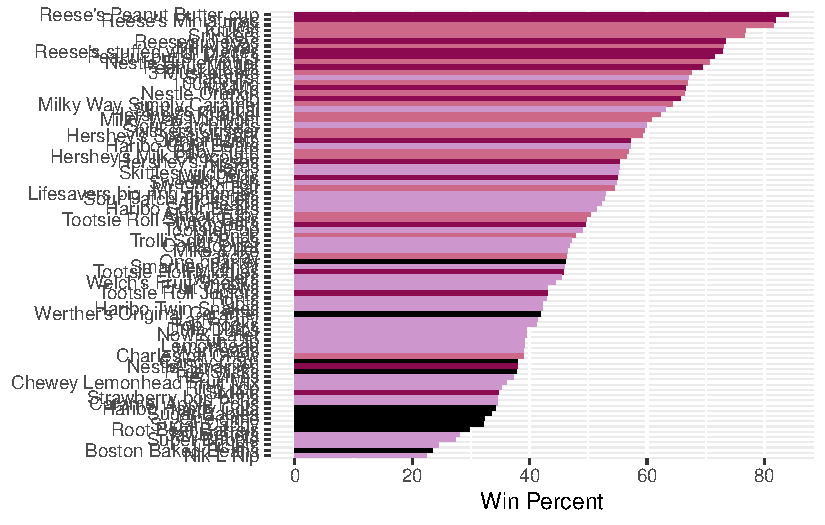
\includegraphics{class07_files/figure-pdf/unnamed-chunk-18-1.pdf}

}

\end{figure}

\begin{Shaded}
\begin{Highlighting}[]
\FunctionTok{barplot}\NormalTok{(}\FunctionTok{as.matrix}\NormalTok{(x), }\AttributeTok{beside=}\NormalTok{F, }\AttributeTok{col=}\FunctionTok{rainbow}\NormalTok{(}\FunctionTok{nrow}\NormalTok{(x)))}
\end{Highlighting}
\end{Shaded}

\begin{figure}[H]

{\centering 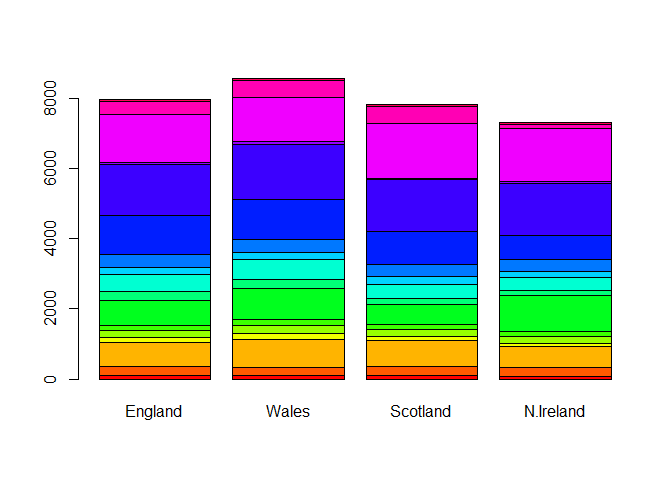
\includegraphics{class07_files/figure-pdf/unnamed-chunk-19-1.pdf}

}

\end{figure}

Changing \texttt{beside=T} to \texttt{beside=F}results in the correct
barplot.

\begin{quote}
Q5: Generating all pairwise plots may help somewhat. Can you make sense
of the following code and resulting figure? What does it mean if a given
point lies on the diagonal for a given plot?
\end{quote}

If a point is on the diagonal, that means the values are all very
similar (i.e.~match the average). If a point is far from that diagonal,
this means it deviates from the norm.

\begin{Shaded}
\begin{Highlighting}[]
\FunctionTok{pairs}\NormalTok{(x, }\AttributeTok{col=}\FunctionTok{rainbow}\NormalTok{(}\DecValTok{10}\NormalTok{), }\AttributeTok{pch=}\DecValTok{16}\NormalTok{)}
\end{Highlighting}
\end{Shaded}

\begin{figure}[H]

{\centering 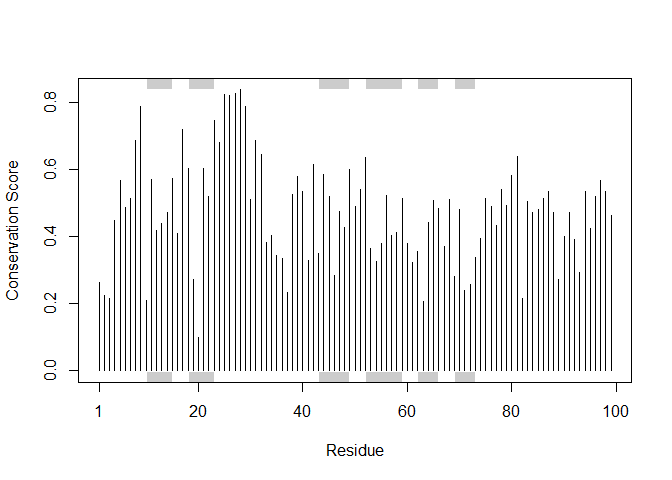
\includegraphics{class07_files/figure-pdf/unnamed-chunk-20-1.pdf}

}

\end{figure}

If a point lies on the diagonal,

\begin{quote}
Q6: What is the main difference between N.Ireland and the other
countries of the UK in terms of this data-set?
\end{quote}

N. Ireland tends to consume less alcoholic beverages and fresh fruit and
consumes more fresh potatoes and soft drinks.

\hypertarget{pca-to-the-rescue}{%
\subsection{PCA to the rescue}\label{pca-to-the-rescue}}

The main ``base'' R function for PCA is called \texttt{prcomp()}. Here
we need to take the transpose of the data to switch the rows and
columns.

\begin{Shaded}
\begin{Highlighting}[]
\NormalTok{pca }\OtherTok{\textless{}{-}} \FunctionTok{prcomp}\NormalTok{( }\FunctionTok{t}\NormalTok{(x) )}
\FunctionTok{summary}\NormalTok{(pca)}
\end{Highlighting}
\end{Shaded}

\begin{verbatim}
Importance of components:
                            PC1      PC2      PC3       PC4
Standard deviation     324.1502 212.7478 73.87622 3.176e-14
Proportion of Variance   0.6744   0.2905  0.03503 0.000e+00
Cumulative Proportion    0.6744   0.9650  1.00000 1.000e+00
\end{verbatim}

\begin{quote}
Q: How much variance is captured in 2 PCs
\end{quote}

96.5\%

To make our main ``PC score plot'' (aka or ``PC1 vs PC2 plot'' or ``PC
plot'' or ``Coordination plot'').

\begin{Shaded}
\begin{Highlighting}[]
\FunctionTok{attributes}\NormalTok{(pca) }
\end{Highlighting}
\end{Shaded}

\begin{verbatim}
$names
[1] "sdev"     "rotation" "center"   "scale"    "x"       

$class
[1] "prcomp"
\end{verbatim}

We are after the \texttt{pca\$x} result component to make our main PCA
plot.

\begin{Shaded}
\begin{Highlighting}[]
\NormalTok{mycols }\OtherTok{\textless{}{-}} \FunctionTok{c}\NormalTok{(}\StringTok{"orange"}\NormalTok{, }\StringTok{"red"}\NormalTok{, }\StringTok{"blue"}\NormalTok{, }\StringTok{"darkgreen"}\NormalTok{)}
\FunctionTok{plot}\NormalTok{(pca}\SpecialCharTok{$}\NormalTok{x[,}\DecValTok{1}\NormalTok{], pca}\SpecialCharTok{$}\NormalTok{x[,}\DecValTok{2}\NormalTok{], }\AttributeTok{col=}\NormalTok{mycols, }\AttributeTok{pch=}\DecValTok{16}\NormalTok{, }\AttributeTok{xlab=}\StringTok{"PC1 (67.4\%)"}\NormalTok{, }\AttributeTok{ylab=}\StringTok{"PC2 (29\%)"}\NormalTok{)}
\end{Highlighting}
\end{Shaded}

\begin{figure}[H]

{\centering 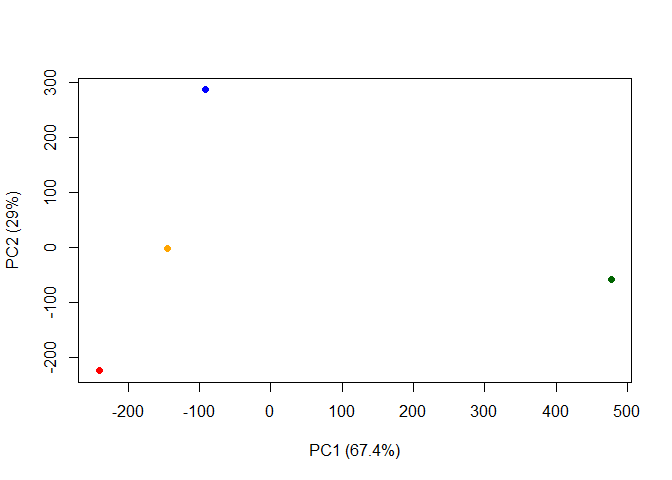
\includegraphics{class07_files/figure-pdf/unnamed-chunk-23-1.pdf}

}

\end{figure}

Another important result from PCA is how the original variables (in this
case: the foods) contribute to the PCs.

This is contained in the \texttt{pca\$rotation} object - folks often
call this the ``loadings'' or ``contributions'' to the PCs.

\begin{Shaded}
\begin{Highlighting}[]
\NormalTok{pca}\SpecialCharTok{$}\NormalTok{rotation}
\end{Highlighting}
\end{Shaded}

\begin{verbatim}
                             PC1          PC2         PC3          PC4
Cheese              -0.056955380  0.016012850  0.02394295 -0.694538519
Carcass_meat         0.047927628  0.013915823  0.06367111  0.489884628
Other_meat          -0.258916658 -0.015331138 -0.55384854  0.279023718
Fish                -0.084414983 -0.050754947  0.03906481 -0.008483145
Fats_and_oils       -0.005193623 -0.095388656 -0.12522257  0.076097502
Sugars              -0.037620983 -0.043021699 -0.03605745  0.034101334
Fresh_potatoes       0.401402060 -0.715017078 -0.20668248 -0.090972715
Fresh_Veg           -0.151849942 -0.144900268  0.21382237 -0.039901917
Other_Veg           -0.243593729 -0.225450923 -0.05332841  0.016719075
Processed_potatoes  -0.026886233  0.042850761 -0.07364902  0.030125166
Processed_Veg       -0.036488269 -0.045451802  0.05289191 -0.013969507
Fresh_fruit         -0.632640898 -0.177740743  0.40012865  0.184072217
Cereals             -0.047702858 -0.212599678 -0.35884921  0.191926714
Beverages           -0.026187756 -0.030560542 -0.04135860  0.004831876
Soft_drinks          0.232244140  0.555124311 -0.16942648  0.103508492
Alcoholic_drinks    -0.463968168  0.113536523 -0.49858320 -0.316290619
Confectionery       -0.029650201  0.005949921 -0.05232164  0.001847469
\end{verbatim}

We can make a plot along PC1.

\begin{Shaded}
\begin{Highlighting}[]
\FunctionTok{library}\NormalTok{(ggplot2)}

\NormalTok{contrib }\OtherTok{\textless{}{-}} \FunctionTok{as.data.frame}\NormalTok{(pca}\SpecialCharTok{$}\NormalTok{rotation)}

\FunctionTok{ggplot}\NormalTok{(contrib) }\SpecialCharTok{+} 
  \FunctionTok{aes}\NormalTok{(PC1, }\FunctionTok{rownames}\NormalTok{(contrib)) }\SpecialCharTok{+}
  \FunctionTok{geom\_col}\NormalTok{()}
\end{Highlighting}
\end{Shaded}

\begin{figure}[H]

{\centering 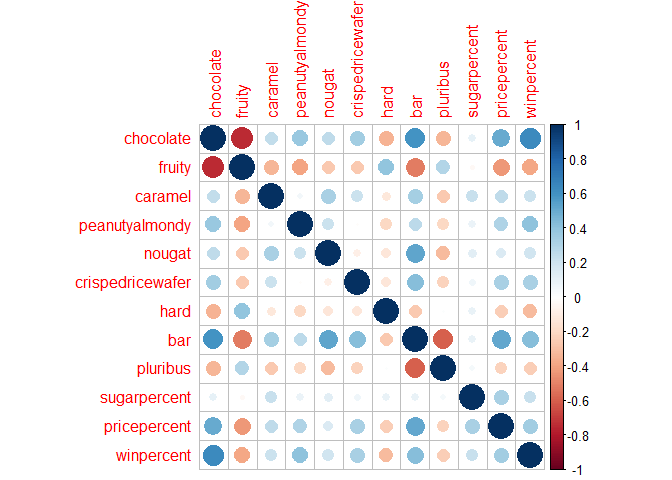
\includegraphics{class07_files/figure-pdf/unnamed-chunk-25-1.pdf}

}

\end{figure}



\end{document}
